\chapter{How He Built a \$200 Million/Year Security Company}

This chapter has to be written with a certain discipline. There is no validated board work to copy, no photographed derivation to transcribe, and no equation visible on screen that we can simply preserve. But the lecture is nevertheless mathematical in a real and useful sense. It is built from partition rules, production targets, deadlines, threshold effects, and a sequence of causal maps. We therefore follow the order in which the speaker unfolds the argument: first the visible outcome, then the scale of the business, then the mechanism of scaling, then the arithmetic of discipline, and finally the deeper model of belief, happiness, and attention.

\begin{remark}
No validated on-screen mathematics survives for this lecture. Every formula and every diagram in what follows is a cautious transcript-based reconstruction, included only where it clarifies a claim the speaker actually makes.
\end{remark}

\section{Status as a Puzzle, Not a Proof}

The lecture begins by showing us the endpoint first: luxury cars, a large house, and an obvious public marker of success. But it does not linger there. The host uses the display only to pose the real question: what did this man do to put himself here? That is the right opening for these notes as well. We do not begin by admiring the result; we begin by asking for its generative structure.

The voiceover then compresses the backstory very quickly. Edwin Arroyave is introduced as someone born in Colombia, brought to the United States as a child, shaped by poverty, foster care, jail in the family, and early household responsibility. Only after that compression do we get the quantitative anchors that make the lecture worth treating as a serious case rather than a lifestyle vignette:
\begin{equation}
t_{\mathrm{security}} = 25\ \text{years},\qquad
a_{\mathrm{start}} = 21,\qquad
a_{\mathrm{now}} = 46,
\end{equation}
together with the business claims
\begin{equation}
R_{\mathrm{life}} > 600\ \text{million dollars},\qquad
R_{\mathrm{year}} \approx 200\ \text{million dollars}.
\end{equation}

These numbers are interview claims, not audited statements. Still, they establish the scale of the object under discussion. The lecture wants us to regard the later rules not as generic motivation, but as the speaker's explanation of how very large outcomes are built.

\section{Influence and the First Step}

Once the host asks how a nine-figure business was scaled, the lecture narrows. The question is no longer who this man is. The question is what mechanism turns a business into a large business. The first answer is strikingly social. It is not technology, product design, or margin structure. It is influence.

The speaker's claim can be written in the following stripped form:
\begin{equation}
\text{Dream large enough for others} + \text{influence}
\Longrightarrow
\text{strong people join}
\Longrightarrow
\text{scale}.
\end{equation}

The lecture insists that good people always have options. So they do not join merely because a slot is open. They join because the leader is credible and because the dream is sufficiently capacious that their own ambitions can fit inside it. That is the first major causal step of the chapter.

But the lecture does not allow this to remain at the level of slogan. It immediately grounds the idea in a memory. When the speaker started the home-security company, he bought the minivan before he had the people to fill it. The action came first; the resources arrived second.

\begin{definition}
In the language of this lecture, faith is not passive assent. It is taking action before one has what one thinks one needs.
\end{definition}

That definition matters because it preserves the order of operations. The point is not merely that one should be hopeful. The point is that one should commit early enough that reality is forced to answer.

\section{Pressure as an Operating Condition}

From the minivan story the speaker moves one step deeper. He says that when money is put behind something, commitment becomes visible. This is where he introduces what he calls a \emph{necessity level}: a sudden willingness that untaps ability one did not know one had.

That move is important. The lecture is now converting a story into an operating rule. Its most compressed statement is:
\begin{equation}
\text{Low stress} \Longrightarrow \text{low performance}.
\end{equation}

We should read this carefully. It is not presented as a laboratory law, nor does the speaker try to quantify optimal stress. What he does claim is that pressure, if voluntarily entered, has a revealing power. It exposes latent effort. It raises urgency. It changes tempo. The lecture therefore presents pressure not as a nuisance to be minimized at all costs, but as an instrument that can raise performance when one is otherwise drifting.

This is also the place where the lecture's rhetoric becomes more deliberate. First comes the principle of influence, then the story of acting before resources, then the law of necessity. In other words, the lecture climbs from scale, to commitment, to pressure.

\section{Focus, Cash Flow, and Diversification}

Only after urgency and commitment have been established does the interview widen into strategic portfolio advice. There is, the host says, a big debate in entrepreneurship: should one diversify early, or should one focus? The speaker answers in favor of sequence.

We may summarize the rule as
\begin{equation}
\text{focus first}
\Longrightarrow
\text{bread-and-butter cash flow}
\Longrightarrow
\text{diversify later}.
\end{equation}

The phrase ``bread and butter'' matters. The lecture is not anti-diversification in principle. Rather, it insists that diversification without a stable engine becomes diffusion. One first becomes genuinely good at one thing, one makes that thing dependable, and only then does one use the surplus structure to move into adjacent domains.

The comparison between security and solar is placed precisely to make this point. The speaker says it took him many years to reach a \$40 million year in security, but only a single year to reach that figure in solar:
\begin{equation}
17\ \text{years in security} \Longrightarrow 40\ \text{million dollars in one year},
\qquad
1\ \text{year in solar} \Longrightarrow 40\ \text{million dollars in one year}.
\end{equation}

The second number is not meant to erase the first. It is meant to depend on it. What looks like speed in the second business is purchased by long apprenticeship in the first. That is one of the lecture's cleanest strategic lessons: leverage belongs to those who have already paid for discipline elsewhere.

\section{Financial Architecture and the First Dream}

The financial advice block turns the lecture from strategy toward arithmetic. Here we move from vague ambition to partition, reserve, and horizon. The speaker says that early on he split every check three ways. One third was for living. One third went to IRS and savings. One third went to a reserve account that, psychologically speaking, did not exist.

We may record the rule as
\begin{equation}
I = I_{\mathrm{live}} + I_{\mathrm{tax+sav}} + I_{\mathrm{res}},
\qquad
I_{\mathrm{live}} = I_{\mathrm{tax+sav}} = I_{\mathrm{res}} = \frac{I}{3}.
\end{equation}

This is one of the lecture's most concrete equations. Its importance is not algebraic complexity. Its importance is sequence. Partition occurs before appetite is allowed to expand.

The following schematic is a transcript-based reconstruction of that rule:

\begin{figure}
\centering
\begin{tikzpicture}[x=1cm,y=1cm]
\draw (0,0) rectangle (3.4,1.2);
\node at (1.7,0.6) {$I_{\mathrm{live}}=\dfrac{I}{3}$};

\draw (4.2,0) rectangle (7.6,1.2);
\node at (5.9,0.6) {$I_{\mathrm{tax+sav}}=\dfrac{I}{3}$};

\draw (8.4,0) rectangle (11.8,1.2);
\node at (10.1,0.6) {$I_{\mathrm{res}}=\dfrac{I}{3}$};

\node at (6.0,2.4) {$I$};
\draw[->] (6.0,2.1)--(1.7,1.2);
\draw[->] (6.0,2.1)--(5.9,1.2);
\draw[->] (6.0,2.1)--(10.1,1.2);
\end{tikzpicture}
\end{figure}

The lecture immediately adds a useful complication. The speaker still wanted nice things. He still wanted to stand out. The thirds rule is therefore not anti-ambition. It is anti-disorder. The lecture is not preaching asceticism. It is trying to show how desire is disciplined so that it can survive shocks.

From here the interview turns to the speaker's first great dream: buying his mother a house. The movement is perfect. Once we have the arithmetic of partition, we are ready for the arithmetic of a concrete promise.

\subsection{Question \& Answer}

\paragraph{Question.} How do we turn a dream into a concrete \(90\)-day blueprint?

\paragraph{Answer.} By forcing the dream to submit to numbers, then to a deadline, and then to a production rate. The speaker gives the data in sequence:
\begin{align}
D &= 12{,}000\ \text{dollars}, &
M &= 1{,}400\ \text{dollars/month}, &
\tau &= 90\ \text{days}, \\
s &\in [8,10]\ \text{sales/week}, &
W &= 12\ \text{weeks}. &&
\end{align}

The lecture does not state the implied total number of sales explicitly, but the reconstruction is straightforward:
\begin{equation}
N = sW \in [96,120]\ \text{sales}.
\end{equation}

We may write the worked calculation out:
\begin{align}
N_{\min} &= 8 \cdot 12 = 96,\\
N_{\max} &= 10 \cdot 12 = 120.
\end{align}

The twelve-week horizon is a planning approximation; it slightly overshoots a literal ninety-day calendar, but it preserves the speaker's structure of thought. The point is not calendar exactness. The point is decomposition.

The lecture's derivation is then:
\begin{enumerate}
\item Fix the target: buy the house for the mother.
\item Read off the immediate constraints \(D\) and \(M\).
\item Place a date on the promise: \(\tau=90\) days.
\item Translate that date into weekly output \(s\).
\item Treat the resulting quota as non-optional.
\item Extend the workday until the required result appears.
\end{enumerate}

This is one of the lecture's clearest moments. A dream ceases to be atmospheric once it has become a count.

The same structure may be summarized visually:

\begin{figure}
\centering
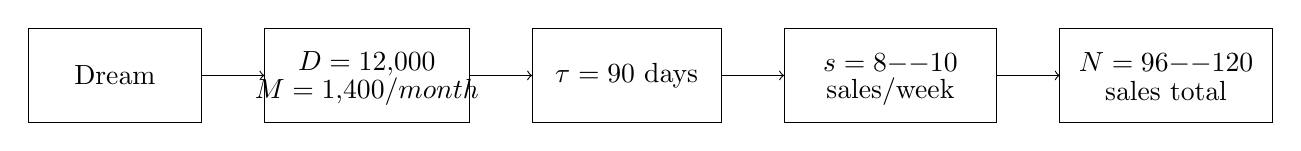
\begin{tikzpicture}[x=1cm,y=1cm]
\draw (0,0) rectangle (2.2,1.2);
\node at (1.1,0.6) {Dream};

\draw (3.0,0) rectangle (5.6,1.2);
\node at (4.3,0.75) {$D=12{,}000$};
\node at (4.3,0.4) {$M=1{,}400/\text{month}$};

\draw (6.4,0) rectangle (8.8,1.2);
\node at (7.6,0.6) {$\tau=90$ days};

\draw (9.6,0) rectangle (12.3,1.2);
\node at (10.95,0.75) {$s=8\text{--}10$};
\node at (10.95,0.4) {sales/week};

\draw (13.1,0) rectangle (15.8,1.2);
\node at (14.45,0.75) {$N=96\text{--}120$};
\node at (14.45,0.4) {sales total};

\draw[->] (2.2,0.6)--(3.0,0.6);
\draw[->] (5.6,0.6)--(6.4,0.6);
\draw[->] (8.8,0.6)--(9.6,0.6);
\draw[->] (12.3,0.6)--(13.1,0.6);
\end{tikzpicture}
\end{figure}

The psychological after-effect is equally important. The speaker says that late-night wins built belief. The arithmetic of the plan changed the emotional posture of the salesman. He no longer appeared desperate because he had internal evidence that a result would come if he stayed in motion.

\section{Scarcity, Hoarding, and the Abundance Formula}

A sponsor interlude interrupts the argument, but when the interview returns it returns with one of its strongest conceptual questions: what separates the middle class from the wealthy? The speaker answers by speaking of a relationship to money.

A bad relationship to money, he says, produces hoarding. Hoarding blocks exposure to the dream. Without contact with the dream, one has little reason to act. Then when difficulty arrives, the accumulated savings are consumed anyway, and the cycle repeats.

We may write the loop in compact form as
\begin{equation}
\text{fear of not enough}
\Longrightarrow
\text{hoarding}
\Longrightarrow
\text{distance from the dream}
\Longrightarrow
\text{weak action}
\Longrightarrow
\text{setback}
\Longrightarrow
\text{fear of not enough}.
\end{equation}

The lecture then offers its counter-model, which the speaker explicitly names as an abundance formula:
\begin{equation}
\text{Become} \to \text{Act} \to \text{Have}.
\end{equation}

The importance lies entirely in the order. One does not first acquire complete safety and then become the kind of person who can act. One becomes first. That is, one begins with hope, faith, and belief. Then one acts before all resources are in hand. Only then does one arrive at having.

The lecture adds a further and very important clause: once action begins, clarity increases. We do not wait for the blueprint in order to move. Rather, the blueprint arrives because we have moved.

The following figure arranges the two sequences side by side:

\begin{figure}
\centering
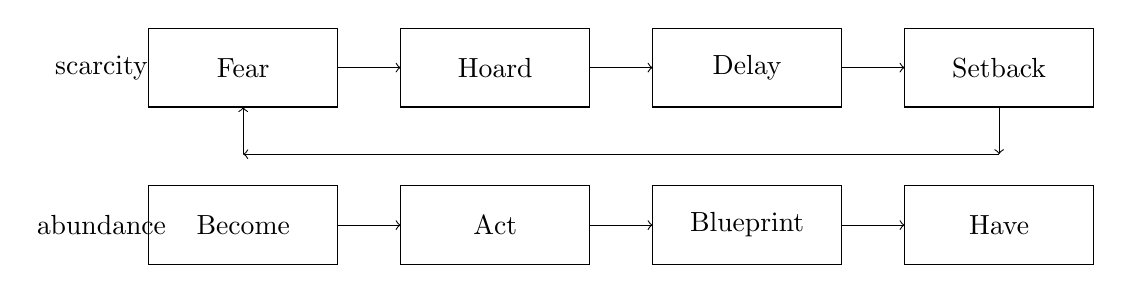
\begin{tikzpicture}[x=1cm,y=1cm]
\node at (-0.6,2.5) {scarcity};
\draw (0,2) rectangle (2.4,3);
\node at (1.2,2.5) {Fear};
\draw (3.2,2) rectangle (5.6,3);
\node at (4.4,2.5) {Hoard};
\draw (6.4,2) rectangle (8.8,3);
\node at (7.6,2.5) {Delay};
\draw (9.6,2) rectangle (12.0,3);
\node at (10.8,2.5) {Setback};

\draw[->] (2.4,2.5)--(3.2,2.5);
\draw[->] (5.6,2.5)--(6.4,2.5);
\draw[->] (8.8,2.5)--(9.6,2.5);
\draw[->] (10.8,2)--(10.8,1.4);
\draw[->] (10.8,1.4)--(1.2,1.4);
\draw[->] (1.2,1.4)--(1.2,2);

\node at (-0.6,0.5) {abundance};
\draw (0,0) rectangle (2.4,1);
\node at (1.2,0.5) {Become};
\draw (3.2,0) rectangle (5.6,1);
\node at (4.4,0.5) {Act};
\draw (6.4,0) rectangle (8.8,1);
\node at (7.6,0.5) {Blueprint};
\draw (9.6,0) rectangle (12.0,1);
\node at (10.8,0.5) {Have};

\draw[->] (2.4,0.5)--(3.2,0.5);
\draw[->] (5.6,0.5)--(6.4,0.5);
\draw[->] (8.8,0.5)--(9.6,0.5);
\end{tikzpicture}
\end{figure}

This is still only the broad outline. The lecture is not content to leave even this formula unqualified. It now asks what blocks action, and what happens when action is met by resistance.

\subsection{Question \& Answer}

\paragraph{Question.} Why does waiting until we have enough money usually keep us stuck?

\paragraph{Answer.} Because waiting is not inert. In the logic of the lecture, waiting changes the person. It makes prudence harden into hoarding, and it makes delay look like wisdom. The counter-order is therefore explicit:
\begin{align}
\text{Become} &= \text{hope} + \text{faith} + \text{belief},\\
\text{Act} &= \text{move before resources are complete},\\
\text{Have} &= \text{the dated result achieved}.
\end{align}

The lecture also insists that action is not followed immediately by reward. It is followed by testing. Just before the blessing, says the speaker, comes the punch. The transcript is slightly garbled in this region, so we keep the formulation modest:
\begin{equation}
\text{Act} \Longrightarrow \text{Test} \Longrightarrow
\begin{cases}
\text{revert to excuses},\\
\text{persist under uncertainty}.
\end{cases}
\end{equation}

That branching point is one of the central structural claims of the lecture. Dates matter, but dates are not enough. Targets matter, but targets are not enough. One must also survive the point at which the plan appears least credible.

\section{Faith, Pleasure, Happiness, and Attention}

From the abundance formula the lecture moves inward. It no longer asks merely how business grows, but how a person organizes the future on the inside. This is why the later material on faith, pleasure, and the reticular activating system is not a digression. It is the lecture's attempt to explain how the earlier operating rules remain psychologically available over long spans of time.

The first interior distinction is between faith and fear:
\begin{align}
\text{Faith} &= \text{projection of the best possible future},\\
\text{Fear} &= \text{projection of the worst possible future}.
\end{align}

The speaker's point is subtle and important. Both are projections. Both concern futures that have not yet happened. The real difference is which future the mind rehearses and therefore prepares itself to recognize.

The second distinction is between pleasure and happiness:
\begin{equation}
\text{Pleasure} = \text{sensation}
\Longrightarrow
\text{pleasure is unstable}.
\end{equation}

This does not mean pleasure is condemned. The speaker explicitly says there is nothing wrong with it. But he does insist that houses, cars, and other exterior factors did not finally give him happiness. They gave pleasure, and pleasure fluctuates. Happiness, in the lecture's vocabulary, becomes more stable when one lives \emph{inside out} rather than \emph{outside in}. The two concrete instruments named here are gratitude and the active conversion of negative events into positive interpretation.

Finally the lecture arrives at a retrospective explanatory model: the reticular activating system. We should present it cautiously. This is not rigorous neuroscience on the page. It is the speaker's way of explaining why dream, self-worth, and survival pressure once seemed to pull opportunities out of the world almost magnetically.

\begin{equation}
\mathrm{RAS}:\ (\text{dreams},\ \text{self-worth},\ \text{survival})
\longmapsto
\text{conscious attention}.
\end{equation}

The following schematic captures the idea at the level needed for these notes:

\begin{figure}
\centering
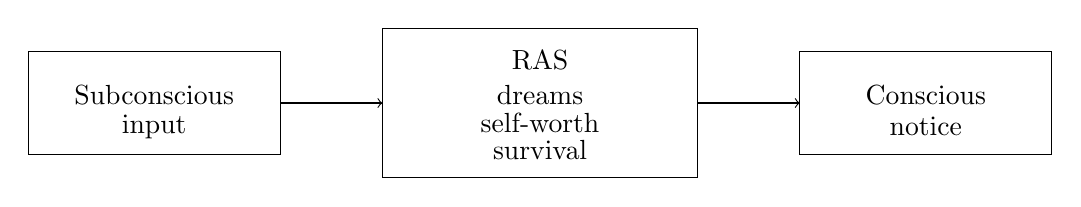
\begin{tikzpicture}[x=1cm,y=1cm]
\draw (0,0.5) rectangle (3.2,1.8);
\node at (1.6,1.25) {Subconscious};
\node at (1.6,0.85) {input};

\draw (4.5,0.2) rectangle (8.5,2.1);
\node at (6.5,1.7) {$\mathrm{RAS}$};
\node at (6.5,1.25) {dreams};
\node at (6.5,0.9) {self-worth};
\node at (6.5,0.55) {survival};

\draw (9.8,0.5) rectangle (13.0,1.8);
\node at (11.4,1.25) {Conscious};
\node at (11.4,0.85) {notice};

\draw[->] (3.2,1.15)--(4.5,1.15);
\draw[->] (8.5,1.15)--(9.8,1.15);
\end{tikzpicture}
\end{figure}

The lecture closes the loop by applying this model backward to the speaker's own life. He says that from youth onward he had already fixed a large dream, a strong sense of self-worth, and a survival-grade need to succeed. On that account, opportunity did not simply appear to him by luck. It became visible because the filter was already tuned to see it.

\section{Summary}

The lecture begins with a house and cars and ends with a theory of attention. Between those two poles it unfolds in a very definite order. First we are shown scale. Then we are told that scale depends on influence. Then influence is made concrete by action before resources. Then pressure is introduced as a performance condition. Then focus is defended against premature diversification. Then income is partitioned, dreams are converted into dates and quotas, and finally the whole structure is reinterpreted through the language of abundance, faith, happiness, and selective notice.

The most useful formulas are simple:
\[
I = \frac{I}{3} + \frac{I}{3} + \frac{I}{3},
\qquad
N = sW \in [96,120],
\qquad
\text{Become} \to \text{Act} \to \text{Have}.
\]
Their simplicity is the point. The lecture is not trying to hide behind complexity. It is trying to insist on order. Dream first, partition second, deadline third, action before completeness, persistence under test, and only then possession. The last turn of the lecture---from faith and fear to attention and self-worth---does not replace the earlier rules. It explains why, for the speaker, those rules could be sustained long enough to matter.